\begin{figure*}
  \centering
  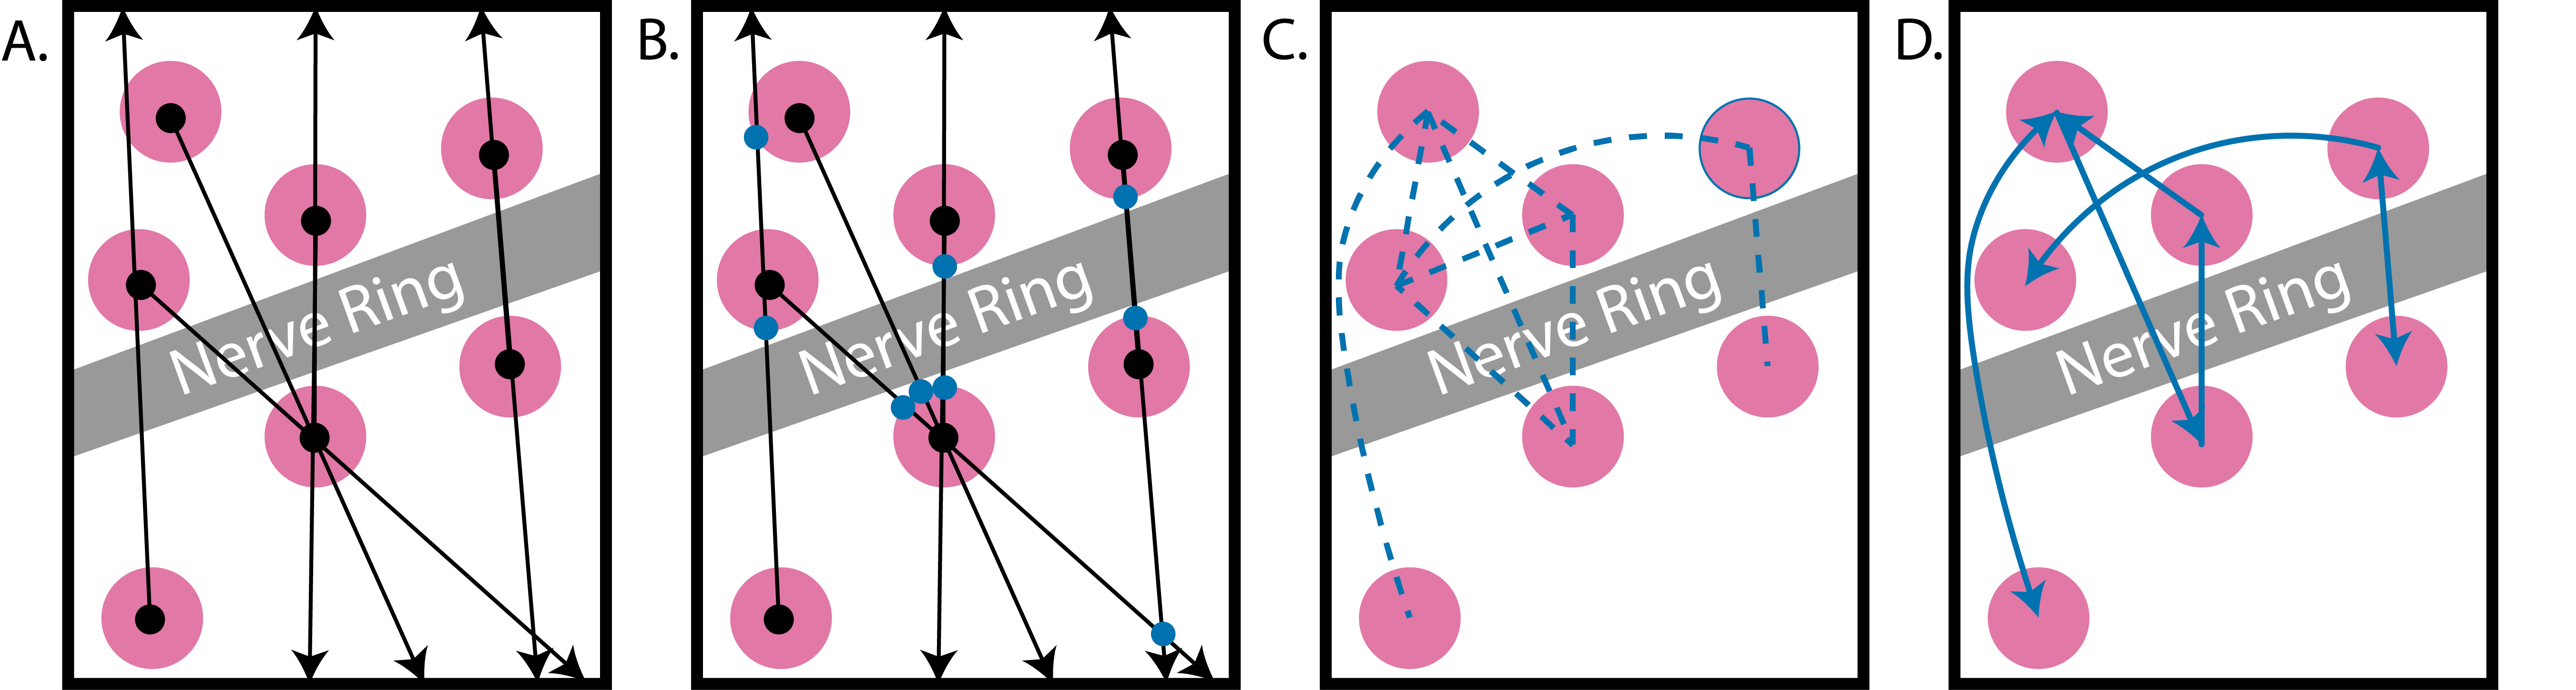
\includegraphics[width=\linewidth]{../data/images/other/SEEM_Method.png}
  \caption{Visual depiction of the Spatially Embedded Edge Model (SEEM) algorithm. 
  \textbf{(A)} For each neuron, SEEM finds the neuron whose soma is closest to it and opposite the Nerve Ring (i.e. the neuron's "penpal"). 
  The algorithm then draws a line segment in 3D space, representative of a neurite, originating in the neuron's soma, extending through the soma of the "penpal," and terminating at the boundaries of the body of \ce. 
  The boundaries are calculated as a range from the minimum coordinate - $\varepsilon$ to the maximum coordinate - $\varepsilon$ for each dimension ($x$,$y$,$z$). $\varepsilon$ is defined as the width of a neurite ($3 \mu m$). 
  \textbf{(B)} If two of these "neurites" are $\le \varepsilon$ away from one another, \textbf{(C)} the two neurons of these neurites form a potential connection. 
  \textbf{(D)} A random subset of these potential connections are chosen equal to the number of total connections found in the \ce network to which it is being compared.}
\end{figure*}